\begin{problem}{태양광 램프}
	{standard input}{standard output}
	{3 seconds}{128 megabytes}{}
	
	
	범수는 크고 아름다운 정원을 가지고 있다. 그는 밤에도 아름다운 광경을 즐기기 위해서 정원에 램프를 설치했다.
	
	이 램프는 방향이 있다. 즉, 이 모든 램프들은 정해진 특정한 각도만 비출 수 있다. 게다가, 범수는 같은 방향을 비추도록 배치를 해 놓았다. 그리고 이 램프는 태양광 램프다. 이상하게도, 배터리가 없는 태양광 패널로 되어있다. 당신은 이 램프가 밤에 비추어야 해서 쓸모 없다고 생각할 수 있지만, 다른 태양광 램프가 이 램프를 비춘다면, 이 램프는 빛을 낼 수 있다.
	
	지금부터 범수는 전기를 공급해서 램프를 키려고 한다. 문제를 간단히 하기 위해, 우리는 램프를 1번부터 $n$번까지 번호를 붙인다. 즉, $i$번 램프는 시간 $i$에 전기가 공급된다. 범수(와 당신)에게 남은 일은, 각 램프가 언제 빛을 비추기 시작하는가이다. 범수에게 이 문제에 대한 답을 알려주는 프로그램을 작성하여라.
	 
	\InputFile
	
	입력의 첫째줄에는 범수가 설치한 램프의 수를 나타내는 정수 $n$이 주어진다. ($1 \le n \le 200,000$) 둘째 줄에는 빛을 비추는 영역을 의미하는 네 개의 정수 $X_1$, $Y_1$, $X_2$, $Y_2$가 공백 하나로 구분되어 주어진다. ($-10^9 \le X_i, Y_i \le 10^9$, $(X_i, Y_i) \neq (0,0)$)
	램프가 $(x, y)$에 배치되어 있다면, $(x, y)$에서 두개의 빛 $(x+X_i, y+Y_i)$이 만드는 각 중 작은 각도에 램프를 비춘다. (경계를 포함하고, 각은 항상 180도 보다 작다. 범수가 실수로 레이저를 사버려서 각이 0도일 수도 있다.)
	
	다음 $n$개의 줄은 $i$번 램프가 $(x_i, y_i)$에 위치해 있다는 것을 나타내는 두 정수 $x_i$와 $y_i$가 공백 하나로 구분되어 주어진다. ($-10^9 \le x_i, y_i \le 10^9$) 어떤 두 램프도 같은 위치에 있지 않다는 것이 보장된다.
	
	다음 줄은 $n$개의 정수 $k_1$, $k_2$, $\cdots$, $k_n$이 공백 하나로 구분되어 주어진다. 이 수는 $i$번째 램프가 $k_i$개의 램프의 빛을 받으면 빛을 내기 시작할 것을 의미한다.

	
	\OutputFile
	프로그램은 첫째 줄에 $n$개의 정수 $t_1$, $t_2$, $\cdots$, $t_n$을 공백 하나로 구분해서 출력해야 한다. 숫자 $t_i$는 $i$번 램프가 시간 $t_i$에 빛을 내기 시작할 것을 의미한다.
	
	\SubtaskWithCost{1}{30}
	\begin{itemize}
		\item $n \le 1000$
	\end{itemize}
	
	\SubtaskWithCost{2}{70}
	
	추가 제한조건이 없다.
	
	\Examples
		
	\begin{example}
	\exmp{
5
3 1 1 3
2 1
1 4
3 4
5 6
5 2
1 2 1 3 2
	}{%
1 2 1 2 5
	}%
	\end{example}
	
	\Note
	
	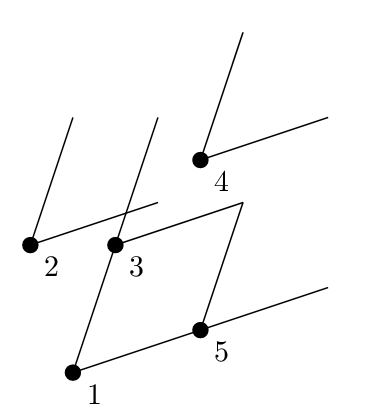
\includegraphics[]{lam.png}
	
	시간 1에 1번 램프를 켜면, 3번 램프도 같이 불이 켜진다. 2번 램프가 켜지면, 4번 램프도 같이 켜진다. (1, 2, 3번 램프가 빛을 비춘다.)
	
\end{problem}

